\documentclass[aspectratio=169,compress]{beamer}
\usepackage{bookmark}
\usepackage{hyperref}
\usetheme{Szeged}
\usecolortheme{beaver}
\graphicspath{ {./figures} }

\newcommand\teeny{\fontsize{3pt}{3.6pt}\selectfont}

\title[\color{white} Billowing Hydrogen]{Billowing Hydrogen}
\subtitle{Simulating Turbulence in HII Regions}
\author[Canales, Wenger]{Eliza Canales \& Trey Wenger}
\institute[UW-Madison \& NRAO]{University of Wisconsin -- Madison \& National Radio Astronomy Observatory}
\date{July 31st, 2024}
\logo{
  
\includegraphics[height=1.25cm]{figures/uwlogo.png}
  \hspace{2mm}
  
\includegraphics[height=1.25cm]{figures/nraologo.png}
}

\setbeamercolor{def}{fg=white,bg=darkred}

\setbeamertemplate{headline}{
  \leavevmode%
  \hbox{\begin{beamercolorbox}[wd=\paperwidth,ht=4.5ex,dp=1.125ex,leftskip=.3cm,rightskip=.3cm]{def}
  \end{beamercolorbox}}
  \vskip0pt%
}
\setbeamertemplate{footline}{
  \leavevmode%
  \hbox{\begin{beamercolorbox}[wd=\paperwidth,ht=4.5ex,dp=1.125ex,leftskip=.3cm,rightskip=.3cm]{def}
  \end{beamercolorbox}}
  \vskip0pt%
}
\setbeamertemplate{navigation symbols}{}

\hypersetup{
    colorlinks=true,
    urlcolor=cyan,
    }
\urlstyle{same}

\begin{document}

\begin{frame}[noframenumbering]
  \titlepage
\end{frame}

\setbeamertemplate{footline}
{%
  \leavevmode%
  \hbox{\begin{beamercolorbox}[wd=.4\paperwidth,ht=4.5ex,dp=1.125ex,leftskip=.3cm,rightskip=.3cm]{def}%
  \insertshorttitle
  \end{beamercolorbox}%
  \begin{beamercolorbox}[wd=.4\paperwidth,ht=4.5ex,dp=1.125ex,leftskip=.3cm,rightskip=.3cm plus1fil]{def}%
    \usebeamerfont{author in head/foot}\insertshortauthor
  \end{beamercolorbox}}%
  \begin{beamercolorbox}[wd=.2\paperwidth,ht=4.5ex,dp=1.125ex,leftskip=.3cm,rightskip=.3cm]{def}%
  \insertshortinstitute\hfill\insertframenumber
  \end{beamercolorbox}%
  \vskip0pt%
}

\begin{frame}{Outline}
  \tableofcontents
\end{frame}

\section{Introduction}
\subsection{HII Regions}
\subsection{How we see them}
\section{Motivations and Project Goals}
\section{Results}
\section{Next Steps}

\begin{frame}
  \frametitle{HII Regions}
  \begin{columns}
    \begin{column}{0.5\textwidth}%%
      \begin{itemize}
        \item What is an HII Region?
        \item Physical Traits
          \begin{itemize}
            \item Powered by hot stars
            \item Can range from AU to parsecs
            \item A type of nebulae
          \end{itemize}
      \end{itemize}
    \end{column}
    \begin{column}{0.5\textwidth}%%
      \teeny
      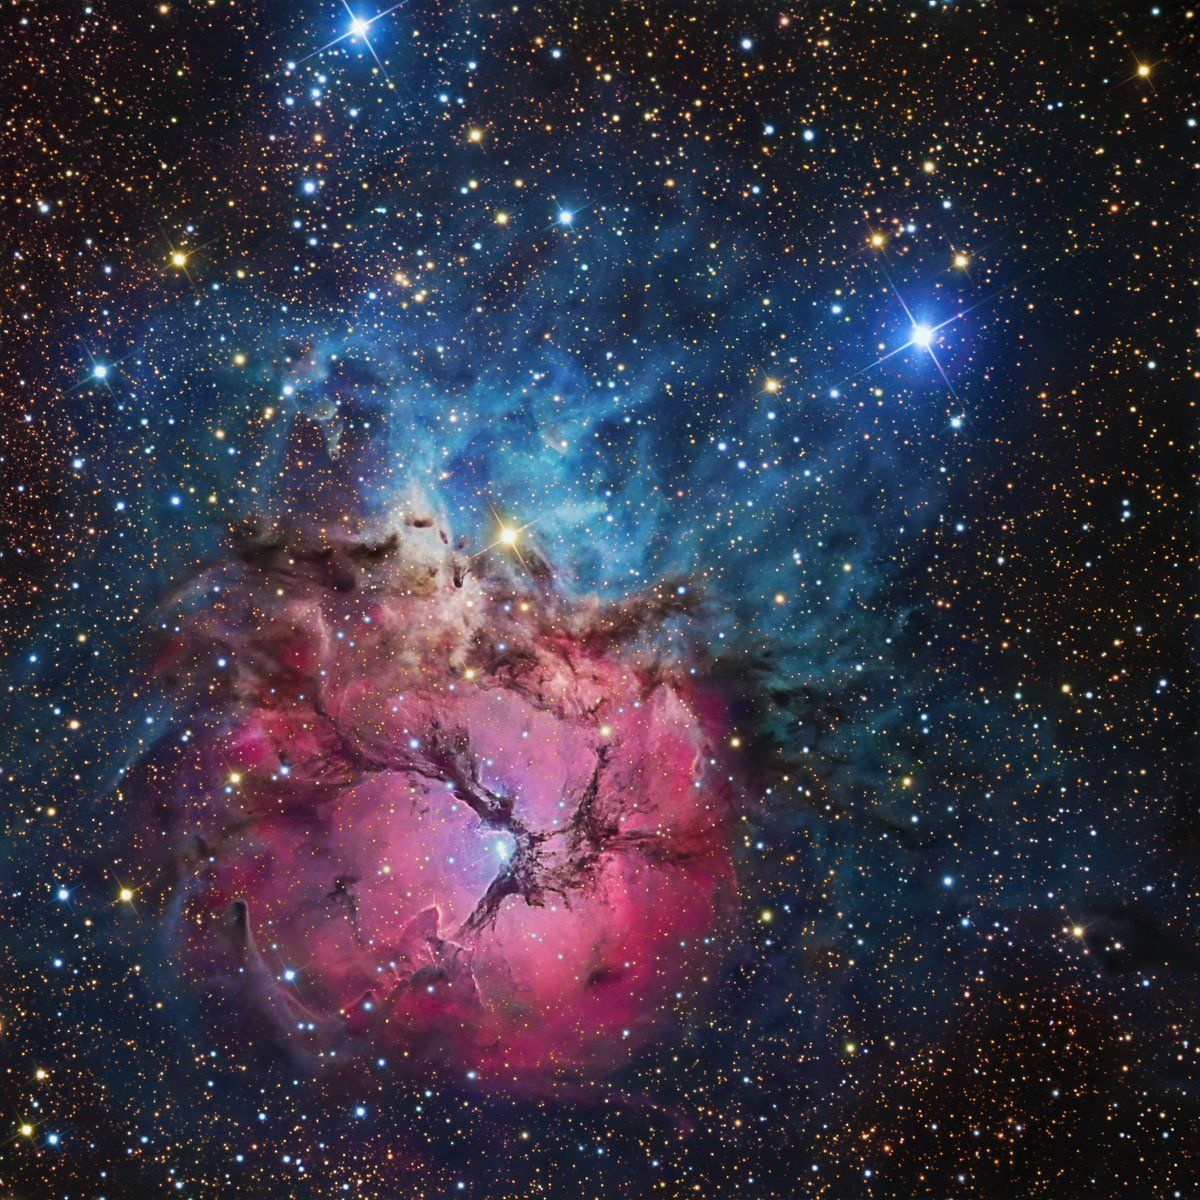
\includegraphics[width=0.7\textwidth]{figures/nebula.jpg}
      {\teeny\\ Image of an HII region, the Trifid Nebula.}
      {\teeny\\ Nebula image: M20 | Trifid Nebula HII Region in Sagittarius 6° from Kaus Borealis (top of the teapot)} 
      {\teeny\\ taken by R Jay GaBany}
      
    \end{column}
  \end{columns}
\end{frame}

\begin{frame}
  \frametitle{Emissions}
  \begin{columns}
    \begin{column}{0.5\textwidth}
      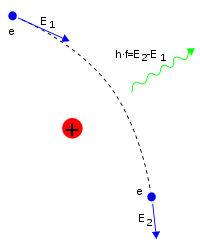
\includegraphics[width=0.35\textwidth]{figures/bremms.png}
      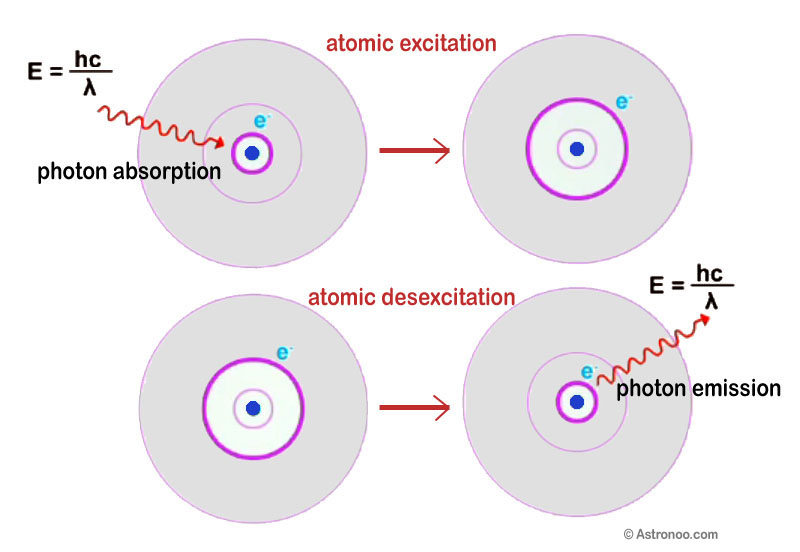
\includegraphics[width=0.55\textwidth]{figures/rrl.jpg}\\
      {\teeny Image 1: Process in which the free-free continuum is created.}
      {\teeny\\ Image 2: Process in which radio recombination lines are created.}
      {\teeny\\ Free-free emission: \url{https://en.wikipedia.org/wiki/Bremsstrahlung\#/media/File:Bremsstrahlung.svg}}
      {\teeny\\ Radio recombination lines: \url{https://astronoo.com/images/lumiere/absorption-et-emission.jpg}}
    \end{column}
    \begin{column}{0.5\textwidth}
      \begin{itemize}
        \item A way we observe HII regions
        \item Why use radio?
        \item Free-free continuum
        \item Radio recombination lines (RRLs)
      \end{itemize}
    \end{column}
  \end{columns}
\end{frame}

\begin{frame}
  \frametitle{Emissions}
  \begin{columns}
    \begin{column}{0.5\textwidth}
      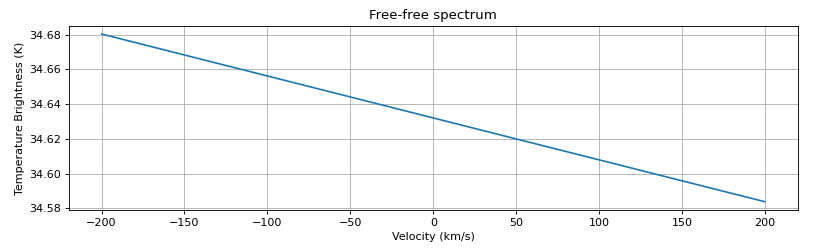
\includegraphics[width=0.8\textwidth]{figures/ffspectrum.png}
      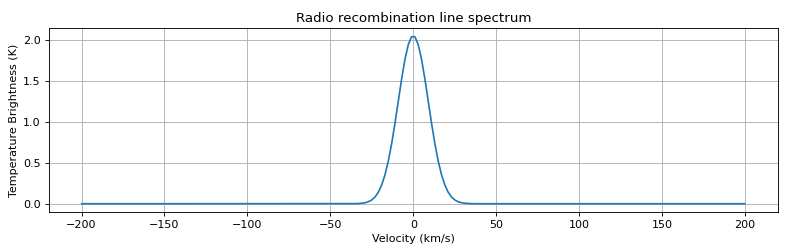
\includegraphics[width=0.8\textwidth]{figures/rrlspectrum.png}
      {\teeny\\ Spectra of free-free emission and a radio recombination line with respect to doppler shift velocity.}
    \end{column}
    \begin{column}{0.5\textwidth}
      \begin{itemize}
        \item A way we observe HII regions
        \item Why use radio?
        \item Free-free continuum
        \item Radio recombination lines (RRLs)
      \end{itemize}
    \end{column}
  \end{columns}
\end{frame}

\begin{frame}
  \frametitle{Radio Imaging}
  \begin{columns}
    \begin{column}{0.5\textwidth}
      \begin{itemize}
        \item Multiple frequencies
        \item Doppler shift
        \item Velocity compared to Local Standard of Rest (VLSR)
        \item Velocity line width
      \end{itemize}
    \end{column}
    \begin{column}{0.5\textwidth}
      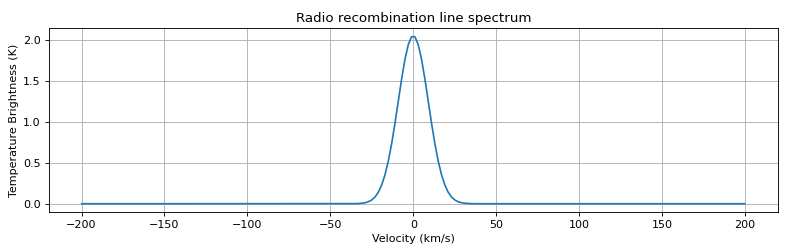
\includegraphics[width=0.8\textwidth]{figures/rrlspectrum.png}
      {\teeny\\ Radio recombination line to discuss how velocity is mapped.}
    \end{column}
  \end{columns}
\end{frame}

\begin{frame}
  \frametitle{Radio Imaging}
  \begin{columns}
    \begin{column}{0.4\textwidth}
      \begin{itemize}
        \item Multiple frequencies
        \item Doppler shift
        \item Velocity compared to Local Standard of Rest (VLSR)
        \item Velocity line width
      \end{itemize}
    \end{column}
    \begin{column}{0.6\textwidth}
      \centering
      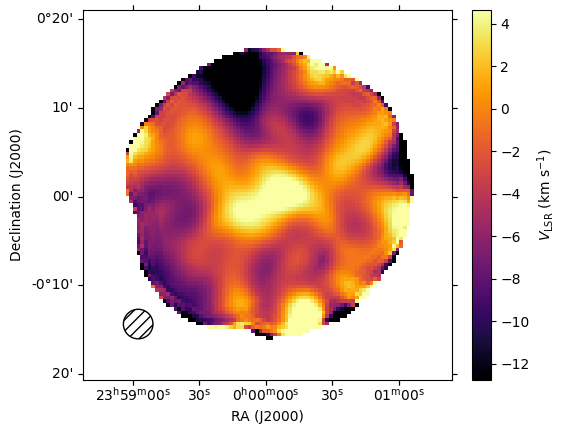
\includegraphics[width=0.45\textwidth]{figures/withdensrrl_200.0_M1.png}
      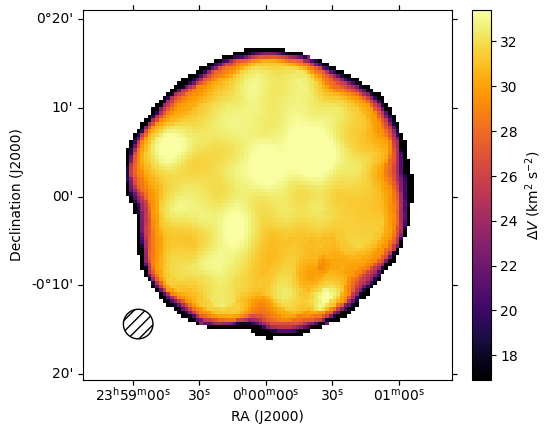
\includegraphics[width=0.45\textwidth]{figures/withdensrrl_200.0_M2.png}
      {\teeny\\ First and second moment maps of an HII region.}
    \end{column}
  \end{columns}
\end{frame}

\begin{frame}
  \frametitle{Emission Line-Broadening}
  \begin{columns}
    \begin{column}{0.3\linewidth}
      \begin{itemize}
        \item Thermal motion
        \item Bulk motion
          \begin{itemize}
            \item Outflow
            \item Expansion
            \item Rotation
          \end{itemize}
        \item Turbulence
      \end{itemize}
    \end{column}
    \begin{column}{0.7\linewidth}
      \centering
      
\includegraphics[height=1in]{figures/fire.png}\\
      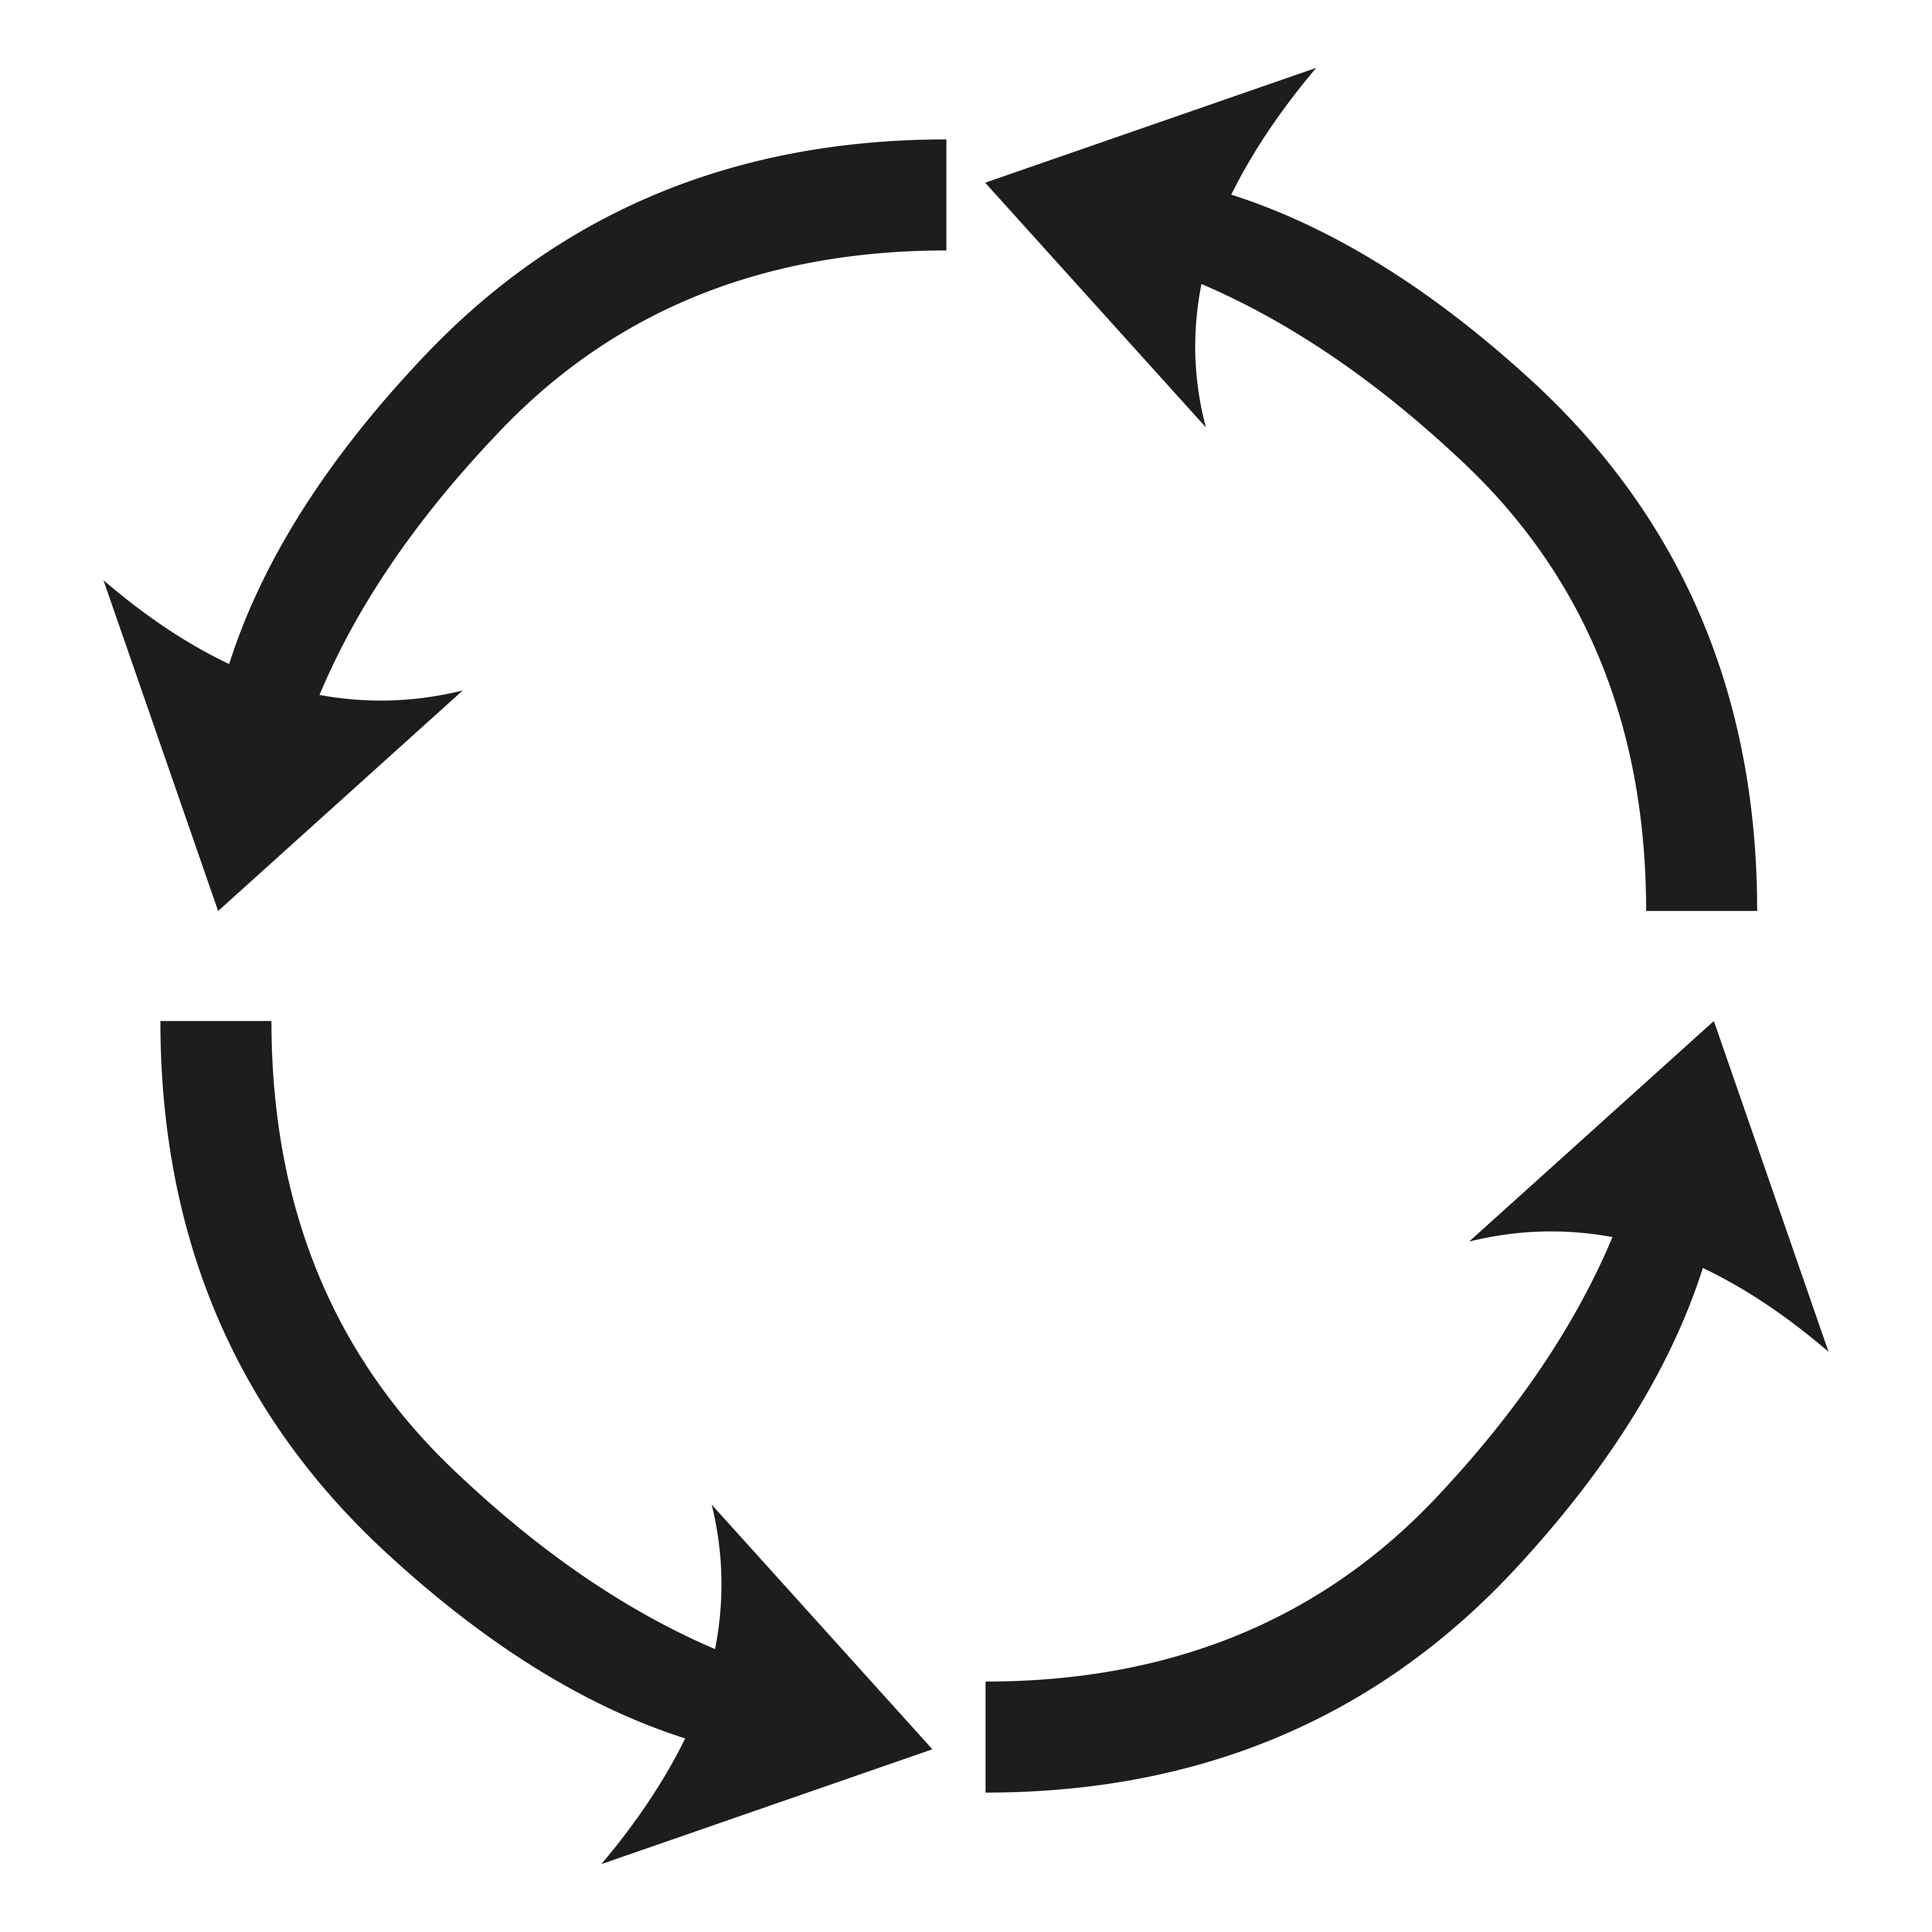
\includegraphics[height=1in]{figures/cycle.png}
      
\includegraphics[height=1in]{figures/wind.png}
      {\teeny\\ Fire: \url{https://www.vecteezy.com/png/19787026-fire-icon-on-transparent-background}}
      {\teeny\\ Cycle: \url{https://www.vecteezy.com/png/18723264-roundabout-directional-arrow-sign-on-transparent-background}}
      {\teeny\\ Wind: \url{https://www.vecteezy.com/png/22183351-hand-drawn-doodle-vaporize-icon}}
    \end{column}
  \end{columns}
\end{frame}

\begin{frame}
  \frametitle{Motivations}
  \begin{itemize}
    \item Previous work had shown what looked like rotation
    \item Later observations show a more complex story
    \item Can turbulence explain this behavior?
  \end{itemize}
  \centering
  \vspace{3mm}
  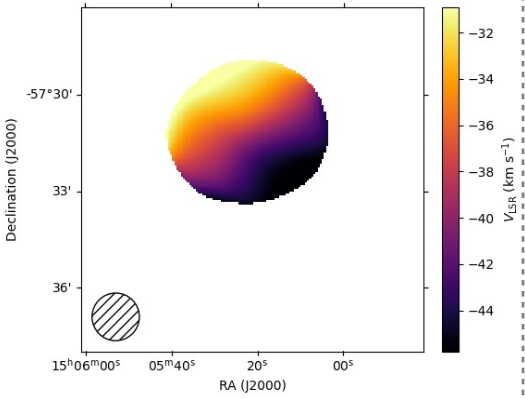
\includegraphics[width=0.3\linewidth]{figures/bigrealVLSR.png}
  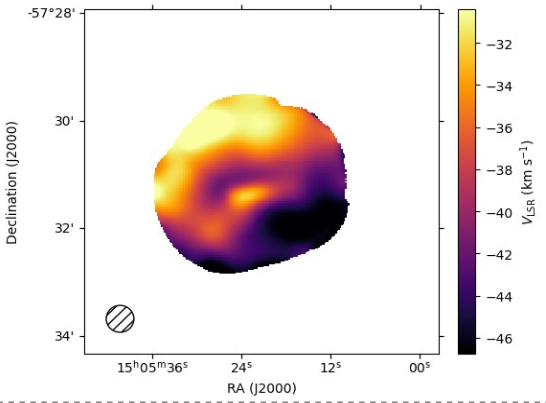
\includegraphics[width=0.3\linewidth]{figures/smallrealVLSR.png}
  {\teeny\\ Showing the how the same object can act differently based on the beam width.}

\end{frame}

\begin{frame}
  \frametitle{Turbulence}
  \begin{columns}
    \begin{column}{0.6\linewidth}
      \centering
      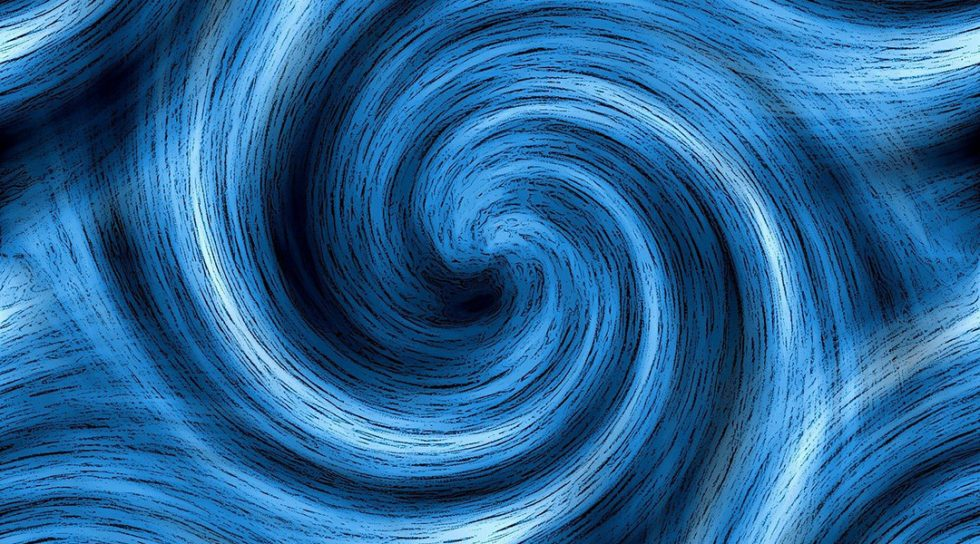
\includegraphics[width=0.8\linewidth]{figures/turbulence.jpg}\\
      {\teeny Image attribution: \url{https://www.advancedsciencenews.com/wp-content/uploads/2023/07/swirl-g52ac5d4ac_1280.jpg}}
    \end{column}
    \begin{column}{0.4\linewidth}
      \begin{itemize}
        \item Hard to model
        \item Not well understood
        \item But can be predicted to a degree!
      \end{itemize}
    \end{column}
  \end{columns}
\end{frame}

\begin{frame}
  \frametitle{Motivations}
  \begin{itemize}
    \item Why not use existing software?
      \begin{itemize}
        \item Similar programs don't use RRLs
        \item Unique problem of density squared
      \end{itemize}
  \end{itemize}
  \centering
  \vspace{3mm}
  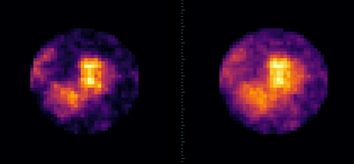
\includegraphics[width=0.5\linewidth]{figures/density_sq.png}
  {\teeny\\ Comparing optically thin tracers, one of density (right) and one of density squared (left).}
\end{frame}

\begin{frame}
  \frametitle{Project Goals}
  \begin{itemize}
    \item Simulate turbulence in HII regions
    \item Test different turbulence parameters
    \item Compare to reality
  \end{itemize}
\end{frame}

\begin{frame}
  \frametitle{Results}
  \centering
  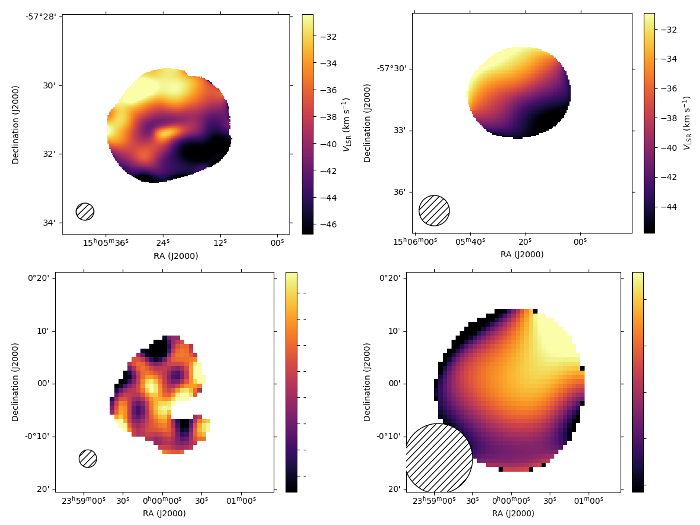
\includegraphics[width=0.5\linewidth]{figures/blurringcomp.png}\\
  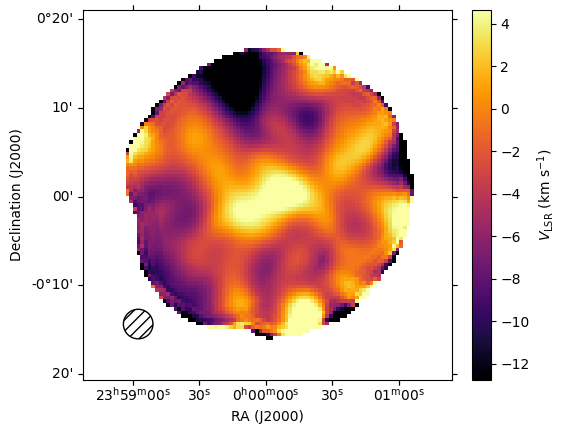
\includegraphics[width=0.25\linewidth]{figures/withdensrrl_200.0_M1.png}
  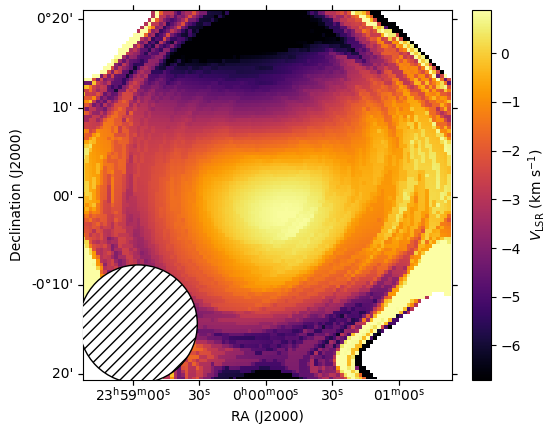
\includegraphics[width=0.25\linewidth]{figures/widerbasicrrl_800.0_M1.png}
  {\teeny\\ Comparing the effects of a higher resolution on the first moment map.}
\end{frame}

\begin{frame}
  \frametitle{Results}
  \begin{columns}
    \begin{column}{0.5\linewidth}
      \begin{itemize}
        \item Similarity to reality
          \begin{itemize}
            \item Turbulence looking like angular momentum
            \item Similar velocity scales
          \end{itemize}
      \end{itemize}
    \end{column}
    \begin{column}{0.5\linewidth}
      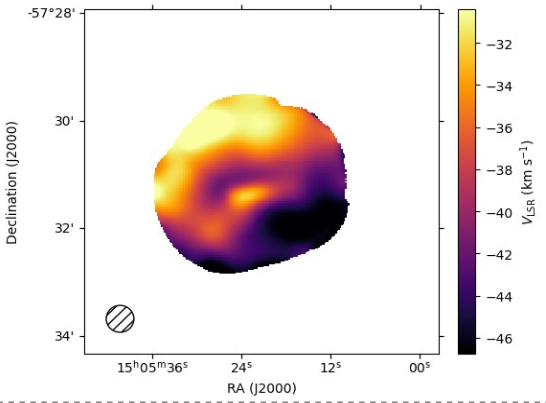
\includegraphics[width=0.6\linewidth]{figures/smallrealVLSR.png}
      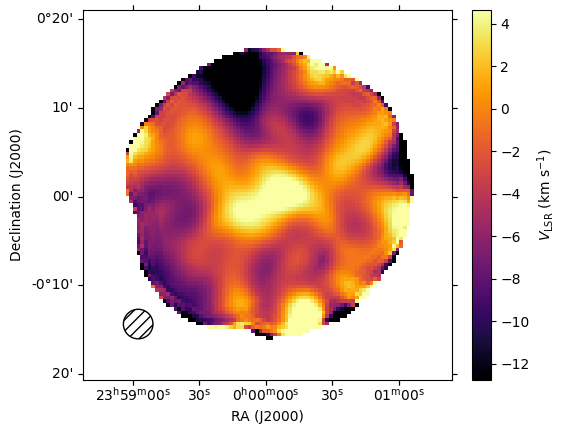
\includegraphics[width=0.6\linewidth]{figures/withdensrrl_200.0_M1.png}
    \end{column}
  \end{columns}
\end{frame}

\begin{frame}
  \frametitle{Future Work}
  \begin{columns}
    \begin{column}{0.5\linewidth}
      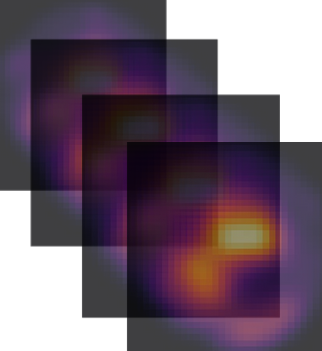
\includegraphics[width=0.7\linewidth]{figures/lagslides.png}
    \end{column}
    \begin{column}{0.5\linewidth}
      \begin{itemize}
        \item Comparing with more radio data
        \item Refining simulation
        \item Testing under various conditions
      \end{itemize}
    \end{column}
  \end{columns}
\end{frame}

\begin{frame}
  \frametitle{Conclusion}
  \begin{itemize}
    \item New data has discrepencies with rotation model
    \item Could turbulence explain HII region behavior?
    \item Tested with simulation
    \item Turbulence is a potential cause for what we see
  \end{itemize}
\end{frame}

\setbeamertemplate{footline}{
  \leavevmode%
  \hbox{\begin{beamercolorbox}[wd=\paperwidth,ht=4.5ex,dp=1.125ex,leftskip=.3cm,rightskip=.3cm]{def}
  \end{beamercolorbox}}
  \vskip0pt%
}

\begin{frame}[noframenumbering]
  \centering
  \Huge
  Thank you!\\
  Any questions?
\end{frame}

\begin{frame}[noframenumbering]
  \frametitle{Pipeline}
  \begin{itemize}
    \item Generate and truncate turbustat data
      \begin{itemize}
        \item Creates cubes to represent density and velocity in 3d space
      \end{itemize}
    \item Calculate emission measure for each physical "voxel" of HII region
    \item Calculate RRL strength for each pixel
      \begin{itemize}
        \item Gaussian treating velocity cube as line centers
        \item Add free-free emission afterwards
      \end{itemize}
  \end{itemize}
\end{frame}

\begin{frame}[noframenumbering]
  \frametitle{Resolution Dependance}
  \centering
  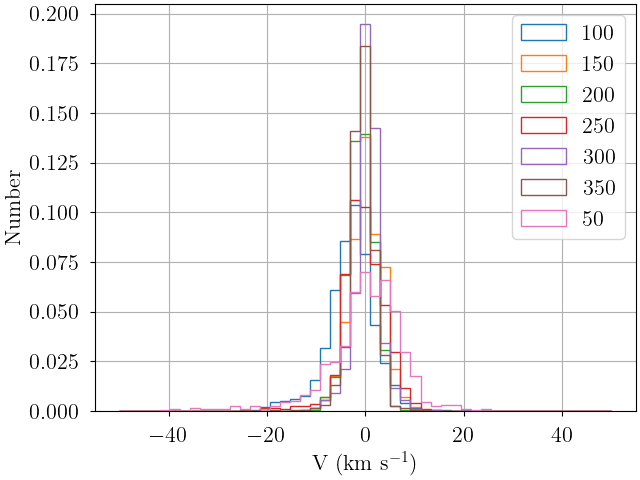
\includegraphics[width=0.6\linewidth]{figures/vel_histogram.png}
  {\teeny\\ Demonstrating that the resolution dependance is negligible past 300 pixels.}
\end{frame}

\end{document}
